\documentclass[border=10pt]{standalone}
\usepackage{pgfplots}
\pgfplotsset{compat=1.18}
\begin{document}
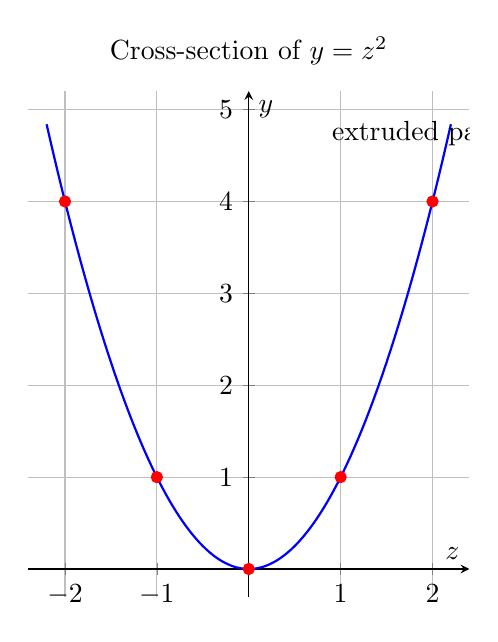
\begin{tikzpicture}
\begin{axis}[
    axis lines=middle,
    xlabel={$z$}, ylabel={$y$},
    title={Cross-section of $y=z^2$},
    domain=-2.2:2.2,
    samples=200,
    grid=major,
    width=10cm,
    height=8cm,
    xmin=-2.4, xmax=2.4,
    ymin=-0.3, ymax=5.2,
    axis equal image,
]
\addplot[blue, thick] {x^2};
\addplot[only marks, red, mark=*] coordinates {(0,0) (1,1) (-1,1) (2,4) (-2,4)};
\node[anchor=south west] at (axis cs:0.8,4.5) {extruded parallel to the $x$-axis};
\end{axis}
\end{tikzpicture}
\end{document}